\documentclass[]{article}
\usepackage{lmodern}
\usepackage{amssymb,amsmath}
\usepackage{ifxetex,ifluatex}
\usepackage{fixltx2e} % provides \textsubscript
\ifnum 0\ifxetex 1\fi\ifluatex 1\fi=0 % if pdftex
  \usepackage[T1]{fontenc}
  \usepackage[utf8]{inputenc}
\else % if luatex or xelatex
  \ifxetex
    \usepackage{mathspec}
  \else
    \usepackage{fontspec}
  \fi
  \defaultfontfeatures{Ligatures=TeX,Scale=MatchLowercase}
\fi
% use upquote if available, for straight quotes in verbatim environments
\IfFileExists{upquote.sty}{\usepackage{upquote}}{}
% use microtype if available
\IfFileExists{microtype.sty}{%
\usepackage{microtype}
\UseMicrotypeSet[protrusion]{basicmath} % disable protrusion for tt fonts
}{}
\usepackage[margin=1in]{geometry}
\usepackage{hyperref}
\hypersetup{unicode=true,
            pdfborder={0 0 0},
            breaklinks=true}
\urlstyle{same}  % don't use monospace font for urls
\usepackage{color}
\usepackage{fancyvrb}
\newcommand{\VerbBar}{|}
\newcommand{\VERB}{\Verb[commandchars=\\\{\}]}
\DefineVerbatimEnvironment{Highlighting}{Verbatim}{commandchars=\\\{\}}
% Add ',fontsize=\small' for more characters per line
\usepackage{framed}
\definecolor{shadecolor}{RGB}{248,248,248}
\newenvironment{Shaded}{\begin{snugshade}}{\end{snugshade}}
\newcommand{\KeywordTok}[1]{\textcolor[rgb]{0.13,0.29,0.53}{\textbf{#1}}}
\newcommand{\DataTypeTok}[1]{\textcolor[rgb]{0.13,0.29,0.53}{#1}}
\newcommand{\DecValTok}[1]{\textcolor[rgb]{0.00,0.00,0.81}{#1}}
\newcommand{\BaseNTok}[1]{\textcolor[rgb]{0.00,0.00,0.81}{#1}}
\newcommand{\FloatTok}[1]{\textcolor[rgb]{0.00,0.00,0.81}{#1}}
\newcommand{\ConstantTok}[1]{\textcolor[rgb]{0.00,0.00,0.00}{#1}}
\newcommand{\CharTok}[1]{\textcolor[rgb]{0.31,0.60,0.02}{#1}}
\newcommand{\SpecialCharTok}[1]{\textcolor[rgb]{0.00,0.00,0.00}{#1}}
\newcommand{\StringTok}[1]{\textcolor[rgb]{0.31,0.60,0.02}{#1}}
\newcommand{\VerbatimStringTok}[1]{\textcolor[rgb]{0.31,0.60,0.02}{#1}}
\newcommand{\SpecialStringTok}[1]{\textcolor[rgb]{0.31,0.60,0.02}{#1}}
\newcommand{\ImportTok}[1]{#1}
\newcommand{\CommentTok}[1]{\textcolor[rgb]{0.56,0.35,0.01}{\textit{#1}}}
\newcommand{\DocumentationTok}[1]{\textcolor[rgb]{0.56,0.35,0.01}{\textbf{\textit{#1}}}}
\newcommand{\AnnotationTok}[1]{\textcolor[rgb]{0.56,0.35,0.01}{\textbf{\textit{#1}}}}
\newcommand{\CommentVarTok}[1]{\textcolor[rgb]{0.56,0.35,0.01}{\textbf{\textit{#1}}}}
\newcommand{\OtherTok}[1]{\textcolor[rgb]{0.56,0.35,0.01}{#1}}
\newcommand{\FunctionTok}[1]{\textcolor[rgb]{0.00,0.00,0.00}{#1}}
\newcommand{\VariableTok}[1]{\textcolor[rgb]{0.00,0.00,0.00}{#1}}
\newcommand{\ControlFlowTok}[1]{\textcolor[rgb]{0.13,0.29,0.53}{\textbf{#1}}}
\newcommand{\OperatorTok}[1]{\textcolor[rgb]{0.81,0.36,0.00}{\textbf{#1}}}
\newcommand{\BuiltInTok}[1]{#1}
\newcommand{\ExtensionTok}[1]{#1}
\newcommand{\PreprocessorTok}[1]{\textcolor[rgb]{0.56,0.35,0.01}{\textit{#1}}}
\newcommand{\AttributeTok}[1]{\textcolor[rgb]{0.77,0.63,0.00}{#1}}
\newcommand{\RegionMarkerTok}[1]{#1}
\newcommand{\InformationTok}[1]{\textcolor[rgb]{0.56,0.35,0.01}{\textbf{\textit{#1}}}}
\newcommand{\WarningTok}[1]{\textcolor[rgb]{0.56,0.35,0.01}{\textbf{\textit{#1}}}}
\newcommand{\AlertTok}[1]{\textcolor[rgb]{0.94,0.16,0.16}{#1}}
\newcommand{\ErrorTok}[1]{\textcolor[rgb]{0.64,0.00,0.00}{\textbf{#1}}}
\newcommand{\NormalTok}[1]{#1}
\usepackage{graphicx,grffile}
\makeatletter
\def\maxwidth{\ifdim\Gin@nat@width>\linewidth\linewidth\else\Gin@nat@width\fi}
\def\maxheight{\ifdim\Gin@nat@height>\textheight\textheight\else\Gin@nat@height\fi}
\makeatother
% Scale images if necessary, so that they will not overflow the page
% margins by default, and it is still possible to overwrite the defaults
% using explicit options in \includegraphics[width, height, ...]{}
\setkeys{Gin}{width=\maxwidth,height=\maxheight,keepaspectratio}
\IfFileExists{parskip.sty}{%
\usepackage{parskip}
}{% else
\setlength{\parindent}{0pt}
\setlength{\parskip}{6pt plus 2pt minus 1pt}
}
\setlength{\emergencystretch}{3em}  % prevent overfull lines
\providecommand{\tightlist}{%
  \setlength{\itemsep}{0pt}\setlength{\parskip}{0pt}}
\setcounter{secnumdepth}{0}
% Redefines (sub)paragraphs to behave more like sections
\ifx\paragraph\undefined\else
\let\oldparagraph\paragraph
\renewcommand{\paragraph}[1]{\oldparagraph{#1}\mbox{}}
\fi
\ifx\subparagraph\undefined\else
\let\oldsubparagraph\subparagraph
\renewcommand{\subparagraph}[1]{\oldsubparagraph{#1}\mbox{}}
\fi

%%% Use protect on footnotes to avoid problems with footnotes in titles
\let\rmarkdownfootnote\footnote%
\def\footnote{\protect\rmarkdownfootnote}

%%% Change title format to be more compact
\usepackage{titling}

% Create subtitle command for use in maketitle
\providecommand{\subtitle}[1]{
  \posttitle{
    \begin{center}\large#1\end{center}
    }
}

\setlength{\droptitle}{-2em}

  \title{}
    \pretitle{\vspace{\droptitle}}
  \posttitle{}
    \author{}
    \preauthor{}\postauthor{}
    \date{}
    \predate{}\postdate{}
  

\begin{document}

\section{Tidyverse}\label{tidyverse}

Adam Rawles

\subsection{Background}\label{background}

\begin{itemize}
\tightlist
\item
  What is the tidyverse?

  \begin{itemize}
  \tightlist
  \item
    A series of packages created by Hadley Wickham
  \item
    Used for data analysis and science
  \item
    All based on an underlying philosophy and structure
  \end{itemize}
\end{itemize}

\subsection{Packages}\label{packages}

\begin{itemize}
\tightlist
\item
  tidyr*
\item
  dplyr*
\item
  stringr*
\item
  ggplot2*
\item
  tibble
\item
  readr
\item
  purrr
\item
  forcats
\end{itemize}

\subsection{Tidy Data}\label{tidy-data}

\begin{itemize}
\tightlist
\item
  A format for datasets

  \begin{itemize}
  \tightlist
  \item
    Each variable in a column
  \item
    Each observation on a row
  \item
    Separate tables for different ``types'' of variables
  \item
    Each related table has a linkable column
  \end{itemize}
\item
  Why use the tidy data format?

  \begin{itemize}
  \tightlist
  \item
    Easier plotting, analysis and manipulation
  \item
    A common format for all datasets
  \item
    Models can be easily translated from one dataset to another
  \end{itemize}
\end{itemize}

\subsection{Tidy Data (example)}\label{tidy-data-example}

\begin{verbatim}
## # A tibble: 3 x 4
##   settlement_date  coal  wind solar
##   <chr>           <dbl> <dbl> <dbl>
## 1 10 Jun 2018       240   120    90
## 2 11 Jun 2018       200   150   100
## 3 12 Jun 2018       190   125    85
\end{verbatim}

\begin{verbatim}
## # A tibble: 9 x 3
##   settlement_date fuel_type output_mwh
##   <chr>           <chr>          <dbl>
## 1 10 Jun 2018     coal             240
## 2 10 Jun 2018     wind             120
## 3 10 Jun 2018     solar             90
## 4 11 Jun 2018     coal             200
## 5 11 Jun 2018     wind             150
## 6 11 Jun 2018     solar            100
## 7 12 Jun 2018     coal             190
## 8 12 Jun 2018     wind             125
## 9 12 Jun 2018     solar             85
\end{verbatim}

\subsection{tidyr}\label{tidyr}

\begin{itemize}
\tightlist
\item
  A package to help with the ``tidying'' process
\item
  Two main groups of functions:

  \begin{itemize}
  \tightlist
  \item
    Tidying (reshaping)
  \item
    Value manipulation
  \end{itemize}
\end{itemize}

\subsection{tidyr - Reshaping}\label{tidyr---reshaping}

\begin{itemize}
\tightlist
\item
  gather()

  \begin{itemize}
  \tightlist
  \item
    Use this function to convert multiple columns into a key and value
    column
  \end{itemize}
\item
  spread()

  \begin{itemize}
  \tightlist
  \item
    Use this function to convert a key column into multiple columns
  \item
    Basically the opposite of gather()
  \end{itemize}
\end{itemize}

\subsection{gather()}\label{gather}

\begin{itemize}
\tightlist
\item
  gather()

  \begin{itemize}
  \tightlist
  \item
    Parameters:

    \begin{itemize}
    \tightlist
    \item
      data: the data frame
    \item
      key: the name of the new ``key'' column
    \item
      value: the name of the new ``value'' column
    \item
      \ldots{}: the columns to be converted
    \end{itemize}
  \end{itemize}
\end{itemize}

\begin{verbatim}
## # A tibble: 3 x 4
##   settlement_date  coal  wind solar
##   <chr>           <dbl> <dbl> <dbl>
## 1 10 Jun 2018       240   120    90
## 2 11 Jun 2018       200   150   100
## 3 12 Jun 2018       190   125    85
\end{verbatim}

\subsection{gather()}\label{gather-1}

\begin{Shaded}
\begin{Highlighting}[]
\NormalTok{untidy_data <-}\StringTok{ }\KeywordTok{tribble}\NormalTok{(}\OperatorTok{~}\NormalTok{settlement_date, }\OperatorTok{~}\NormalTok{coal, }\OperatorTok{~}\NormalTok{wind, }\OperatorTok{~}\NormalTok{solar,}
                    \StringTok{"10 Jun 2018"}\NormalTok{, }\DecValTok{240}\NormalTok{, }\DecValTok{120}\NormalTok{, }\DecValTok{90}\NormalTok{,}
                    \StringTok{"11 Jun 2018"}\NormalTok{, }\DecValTok{200}\NormalTok{, }\DecValTok{150}\NormalTok{, }\DecValTok{100}\NormalTok{,}
                    \StringTok{"12 Jun 2018"}\NormalTok{, }\DecValTok{190}\NormalTok{, }\DecValTok{125}\NormalTok{, }\DecValTok{85}\NormalTok{)}

\NormalTok{tidy_data <-}\StringTok{ }\KeywordTok{gather}\NormalTok{(untidy_data, }\DataTypeTok{key =} \StringTok{"fuel_type"}\NormalTok{, }\DataTypeTok{value =} \StringTok{"output_mwh"}\NormalTok{, coal}\OperatorTok{:}\NormalTok{solar) }\CommentTok{#we could also use c(coal, wind, solar)}

\NormalTok{tidy_data}
\end{Highlighting}
\end{Shaded}

\begin{verbatim}
## # A tibble: 9 x 3
##   settlement_date fuel_type output_mwh
##   <chr>           <chr>          <dbl>
## 1 10 Jun 2018     coal             240
## 2 11 Jun 2018     coal             200
## 3 12 Jun 2018     coal             190
## 4 10 Jun 2018     wind             120
## 5 11 Jun 2018     wind             150
## 6 12 Jun 2018     wind             125
## 7 10 Jun 2018     solar             90
## 8 11 Jun 2018     solar            100
## 9 12 Jun 2018     solar             85
\end{verbatim}

\subsection{gather() - exercise}\label{gather---exercise}

\begin{itemize}
\tightlist
\item
  Import the .csv file I sent you
\item
  Convert it to the tidy data format
\end{itemize}

\subsection{tidyr - value
manipulation}\label{tidyr---value-manipulation}

\begin{itemize}
\tightlist
\item
  You can also use tidyr to handle missing values, and split or
  concatenate cells
\item
  Missing values

  \begin{itemize}
  \tightlist
  \item
    drop\_na(data, \ldots{}) removes all rows with NA in \ldots{}
    columns
  \item
    fill(data, \ldots{}) replaces all NAs with most recent values in
    \ldots{}columns
  \item
    replace\_na(data, replace, \ldots{}) replaces all NAs with the
    values in replace in \ldots{}columns
  \end{itemize}
\item
  Split/join

  \begin{itemize}
  \tightlist
  \item
    seperate/\_rows(data, col, into, sep) separates values into several
    columns/rows
  \item
    unite(data, col, \ldots{}, sep) unites \ldots{}columns into a single
    column with a separator
  \end{itemize}
\end{itemize}

\subsection{tidyr - value manipulation
example}\label{tidyr---value-manipulation-example}

\begin{Shaded}
\begin{Highlighting}[]
\KeywordTok{unite}\NormalTok{(untidy_data, coal, solar, wind, }\DataTypeTok{col =} \StringTok{"coal_solar_wind"}\NormalTok{, }\DataTypeTok{sep =} \StringTok{"/"}\NormalTok{,  )}
\end{Highlighting}
\end{Shaded}

\begin{verbatim}
## # A tibble: 3 x 2
##   settlement_date coal_solar_wind
##   <chr>           <chr>          
## 1 10 Jun 2018     240/90/120     
## 2 11 Jun 2018     200/100/150    
## 3 12 Jun 2018     190/85/125
\end{verbatim}

\subsection{dplyr}\label{dplyr}

\begin{itemize}
\tightlist
\item
  So now you've got your raw tidy data
\item
  The next step is data manipulation

  \begin{itemize}
  \tightlist
  \item
    aggregate
  \item
    calculated columns
  \item
    subset
  \end{itemize}
\item
  All of these can be done with the dplyr package
\end{itemize}

\subsection{dplyr - the pipe \%\textgreater{}\%}\label{dplyr---the-pipe}

\begin{itemize}
\tightlist
\item
  The pipe passes the evaluated result of a function on the left of the
  pipe as the first argument to the function on the right
\item
  Example
\end{itemize}

\begin{Shaded}
\begin{Highlighting}[]
\KeywordTok{library}\NormalTok{(tidyverse)}

\KeywordTok{sum}\NormalTok{(}\KeywordTok{c}\NormalTok{(}\DecValTok{1}\NormalTok{,}\DecValTok{2}\NormalTok{,}\DecValTok{3}\NormalTok{,}\DecValTok{4}\NormalTok{)) }\OperatorTok\StringTok{ }\KeywordTok{print}\NormalTok{()}
\end{Highlighting}
\end{Shaded}

\begin{verbatim}
## [1] 10
\end{verbatim}

\begin{Shaded}
\begin{Highlighting}[]
\StringTok{"hello"} \OperatorTok\StringTok{ }\KeywordTok{substr}\NormalTok{(}\DecValTok{1}\NormalTok{,}\DecValTok{2}\NormalTok{)}
\end{Highlighting}
\end{Shaded}

\begin{verbatim}
## [1] "he"
\end{verbatim}

\subsection{dplyr - the pipe
\%\textgreater{}\%}\label{dplyr---the-pipe-1}

\begin{itemize}
\tightlist
\item
  This can be very useful when performing multiple manipulation steps

  \begin{itemize}
  \tightlist
  \item
    e.g.~grouping, then finding an average, then subsetting, etc.
  \item
    It also allows you to read from left to right, rather than from
    inside to outside if the function calls were embedded\ldots{}
  \end{itemize}
\end{itemize}

\begin{Shaded}
\begin{Highlighting}[]
\KeywordTok{sum}\NormalTok{(}\KeywordTok{c}\NormalTok{(}\DecValTok{1}\NormalTok{,}\DecValTok{2}\NormalTok{,}\DecValTok{3}\NormalTok{,}\DecValTok{4}\NormalTok{)) }\OperatorTok\StringTok{ }\KeywordTok{print}\NormalTok{()}
\end{Highlighting}
\end{Shaded}

\begin{verbatim}
## [1] 10
\end{verbatim}

\begin{Shaded}
\begin{Highlighting}[]
\KeywordTok{print}\NormalTok{(}\KeywordTok{sum}\NormalTok{(}\KeywordTok{c}\NormalTok{(}\DecValTok{1}\NormalTok{,}\DecValTok{2}\NormalTok{,}\DecValTok{3}\NormalTok{,}\DecValTok{4}\NormalTok{)))}
\end{Highlighting}
\end{Shaded}

\begin{verbatim}
## [1] 10
\end{verbatim}

\subsection{dplyr - the pipe
\%\textgreater{}\%}\label{dplyr---the-pipe-2}

\begin{itemize}
\tightlist
\item
  If you don't want the evaulated result to be passed as the first
  argument, you can use a full stop (``.'') to specify which parameter
  you want the result passed as\ldots{}
\end{itemize}

\begin{Shaded}
\begin{Highlighting}[]
\DecValTok{2} \OperatorTok\StringTok{ }\KeywordTok{substr}\NormalTok{(}\StringTok{"hello"}\NormalTok{, ., }\DecValTok{4}\NormalTok{)}
\end{Highlighting}
\end{Shaded}

\begin{verbatim}
## [1] "ell"
\end{verbatim}

\subsection{dplyr - aggregate}\label{dplyr---aggregate}

\begin{itemize}
\tightlist
\item
  summarise()

  \begin{itemize}
  \tightlist
  \item
    This is the main aggregation function
  \item
    Parameters

    \begin{itemize}
    \tightlist
    \item
      .data: the data frame to be summarised
    \item
      \ldots{} name-value pairs of summary functions

      \begin{itemize}
      \tightlist
      \item
        This defines what type of summary we want to do
      \end{itemize}
    \end{itemize}
  \end{itemize}
\end{itemize}

\subsection{dplyr - summarise()
example}\label{dplyr---summarise-example}

\begin{Shaded}
\begin{Highlighting}[]
\NormalTok{output_data <-}\StringTok{ }\NormalTok{tibble}\OperatorTok{::}\KeywordTok{tribble}\NormalTok{(}\OperatorTok{~}\NormalTok{settlement_date, }\OperatorTok{~}\NormalTok{fuel_type, }\OperatorTok{~}\NormalTok{output_mwh,}
                \StringTok{"10 Jun 2018"}\NormalTok{, }\StringTok{"coal"}\NormalTok{, }\DecValTok{240}\NormalTok{,}
                \StringTok{"10 Jun 2018"}\NormalTok{, }\StringTok{"wind"}\NormalTok{, }\DecValTok{120}\NormalTok{,}
                \StringTok{"10 Jun 2018"}\NormalTok{, }\StringTok{"solar"}\NormalTok{, }\DecValTok{90}\NormalTok{,}
                \StringTok{"11 Jun 2018"}\NormalTok{, }\StringTok{"coal"}\NormalTok{, }\DecValTok{200}\NormalTok{,}
                \StringTok{"11 Jun 2018"}\NormalTok{, }\StringTok{"wind"}\NormalTok{, }\DecValTok{150}\NormalTok{,}
                \StringTok{"11 Jun 2018"}\NormalTok{, }\StringTok{"solar"}\NormalTok{, }\DecValTok{100}\NormalTok{,}
                \StringTok{"12 Jun 2018"}\NormalTok{, }\StringTok{"coal"}\NormalTok{, }\DecValTok{190}\NormalTok{,}
                \StringTok{"12 Jun 2018"}\NormalTok{, }\StringTok{"wind"}\NormalTok{, }\DecValTok{125}\NormalTok{,}
                \StringTok{"12 Jun 2018"}\NormalTok{, }\StringTok{"solar"}\NormalTok{, }\DecValTok{85}\NormalTok{)}

\NormalTok{output_data }\OperatorTok\StringTok{ }\KeywordTok{summarise}\NormalTok{(}\DataTypeTok{output_mean =} \KeywordTok{mean}\NormalTok{(output_mwh))}
\end{Highlighting}
\end{Shaded}

\begin{verbatim}
## # A tibble: 1 x 1
##   output_mean
##         <dbl>
## 1        144.
\end{verbatim}

\subsection{dplyr - summarise() by
group}\label{dplyr---summarise-by-group}

\begin{itemize}
\tightlist
\item
  Alone, this functionality isn't particularly powerful
\item
  However, when you combine with the group\_by() function, you can
  produce more useful summaries
\item
  The group\_by() function does exactly what it says: it groups the
  values based a key field
\end{itemize}

\begin{Shaded}
\begin{Highlighting}[]
\NormalTok{output_data }\OperatorTok\StringTok{ }\KeywordTok{group_by}\NormalTok{(settlement_date) }\OperatorTok\StringTok{ }\KeywordTok{summarise}\NormalTok{(}\DataTypeTok{output_mean =} \KeywordTok{mean}\NormalTok{(output_mwh))}
\end{Highlighting}
\end{Shaded}

\begin{verbatim}
## # A tibble: 3 x 2
##   settlement_date output_mean
##   <chr>                 <dbl>
## 1 10 Jun 2018            150 
## 2 11 Jun 2018            150 
## 3 12 Jun 2018            133.
\end{verbatim}

\begin{itemize}
\tightlist
\item
  This is similar to the aggregate functions and group by clauses in SQL
\end{itemize}

\subsection{dplyr - calculated
columns}\label{dplyr---calculated-columns}

\begin{itemize}
\tightlist
\item
  Another feature of the dplyr package is the ability to produce
  calculated columns more easily
\item
  The mutate() function does this for us
\end{itemize}

\subsection{dplyr - mutate()}\label{dplyr---mutate}

\begin{itemize}
\tightlist
\item
  mutate()

  \begin{itemize}
  \tightlist
  \item
    Parameters

    \begin{itemize}
    \tightlist
    \item
      .data: the data frame to which the column will be added
    \item
      \ldots{}: name-value pairs of expressions. Name will be the column
      name and value will be the calculated value
    \end{itemize}
  \end{itemize}
\end{itemize}

\section{dplyr - mutate() example}\label{dplyr---mutate-example}

\begin{Shaded}
\begin{Highlighting}[]
\NormalTok{output_data }\OperatorTok\StringTok{ }\KeywordTok{mutate}\NormalTok{(}\DataTypeTok{cum_output =} \KeywordTok{cumsum}\NormalTok{(output_mwh))}
\end{Highlighting}
\end{Shaded}

\begin{verbatim}
## # A tibble: 9 x 4
##   settlement_date fuel_type output_mwh cum_output
##   <chr>           <chr>          <dbl>      <dbl>
## 1 10 Jun 2018     coal             240        240
## 2 10 Jun 2018     wind             120        360
## 3 10 Jun 2018     solar             90        450
## 4 11 Jun 2018     coal             200        650
## 5 11 Jun 2018     wind             150        800
## 6 11 Jun 2018     solar            100        900
## 7 12 Jun 2018     coal             190       1090
## 8 12 Jun 2018     wind             125       1215
## 9 12 Jun 2018     solar             85       1300
\end{verbatim}

\subsection{dplyr - mutate() example}\label{dplyr---mutate-example-1}

\begin{itemize}
\tightlist
\item
  With a group\_by() clause\ldots{}
\end{itemize}

\begin{Shaded}
\begin{Highlighting}[]
\NormalTok{output_data }\OperatorTok\StringTok{ }\KeywordTok{group_by}\NormalTok{(fuel_type) }\OperatorTok\StringTok{ }\KeywordTok{mutate}\NormalTok{(}\DataTypeTok{cum_output =} \KeywordTok{cumsum}\NormalTok{(output_mwh))}
\end{Highlighting}
\end{Shaded}

\begin{verbatim}
## # A tibble: 9 x 4
## # Groups:   fuel_type [3]
##   settlement_date fuel_type output_mwh cum_output
##   <chr>           <chr>          <dbl>      <dbl>
## 1 10 Jun 2018     coal             240        240
## 2 10 Jun 2018     wind             120        120
## 3 10 Jun 2018     solar             90         90
## 4 11 Jun 2018     coal             200        440
## 5 11 Jun 2018     wind             150        270
## 6 11 Jun 2018     solar            100        190
## 7 12 Jun 2018     coal             190        630
## 8 12 Jun 2018     wind             125        395
## 9 12 Jun 2018     solar             85        275
\end{verbatim}

\subsection{dplyr - exercise}\label{dplyr---exercise}

\begin{itemize}
\tightlist
\item
  Using your tidied data set\ldots{}
\item
  Create a new column of the next value (lead()), grouped by
  consumption/generation
\item
  Summarise the dataset (your choice of function) by settlement date
\end{itemize}

\subsection{stringr}\label{stringr}

\begin{itemize}
\tightlist
\item
  We won't go into much detail here today
\item
  stringr is a package for string manipulation
\item
  It uses the regex language (which stands for regular expression) in
  its functions

  \begin{itemize}
  \tightlist
  \item
    This language allows us to search for very specific character
    patterns
  \end{itemize}
\item
  TL;DR Use this package if you ever need to search for text or for an
  expression
\end{itemize}

\subsection{ggplot2}\label{ggplot2}

\begin{itemize}
\tightlist
\item
  ggplot2 is a powerful graphing package
\item
  It's based on a philosophy called The Grammar of Graphics

  \begin{itemize}
  \tightlist
  \item
    A plot is made up of a number of parts

    \begin{itemize}
    \tightlist
    \item
      The data, and its mapping to the plot area (which data goes on the
      X and which data goes on the Y)
    \item
      Geometric objects (do we want to use lines, or bars, or points, or
      whatever)
    \item
      The scales, titles, legends, etc (often collectively termed
      ``scale'')
    \end{itemize}
  \item
    The data and the geometric objects together form a layer, and a plot
    can have many layers
  \end{itemize}
\end{itemize}

\subsection{ggplot2 - layer}\label{ggplot2---layer}

\begin{itemize}
\tightlist
\item
  To create a layer, we need a data set, our mappings, and our objects
\item
  To do this, we employ ggplot2's hierarchical structure
\item
  First, we start with the ggplot() function where we define our dataset
  and optionally your aesthetics\ldots{}
\end{itemize}

\begin{Shaded}
\begin{Highlighting}[]
\KeywordTok{ggplot}\NormalTok{(}\DataTypeTok{data =}\NormalTok{ output_data, }\KeywordTok{aes}\NormalTok{(}\DataTypeTok{x =}\NormalTok{ settlement_date, }\DataTypeTok{y =}\NormalTok{ output_mwh))}
\end{Highlighting}
\end{Shaded}

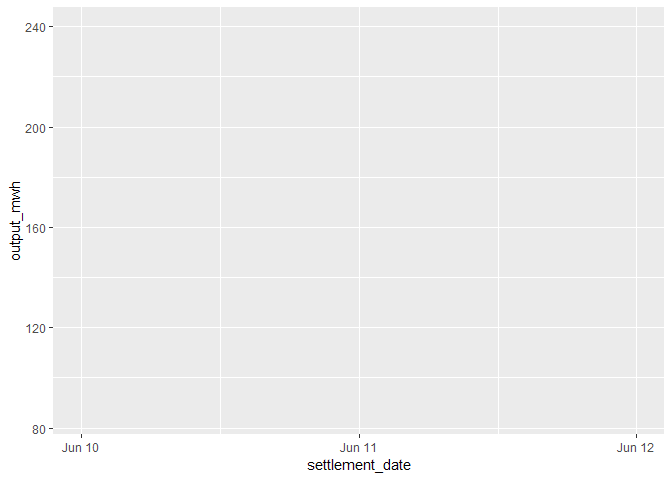
\includegraphics{r_training_tidyverse_files/figure-latex/ggplot2_data-1.pdf}

\subsection{ggplot2 - layer}\label{ggplot2---layer-1}

\begin{Shaded}
\begin{Highlighting}[]
\KeywordTok{ggplot}\NormalTok{(}\DataTypeTok{data =}\NormalTok{ output_data, }\KeywordTok{aes}\NormalTok{(}\DataTypeTok{x =}\NormalTok{ settlement_date, }\DataTypeTok{y =}\NormalTok{ output_mwh))}
\end{Highlighting}
\end{Shaded}

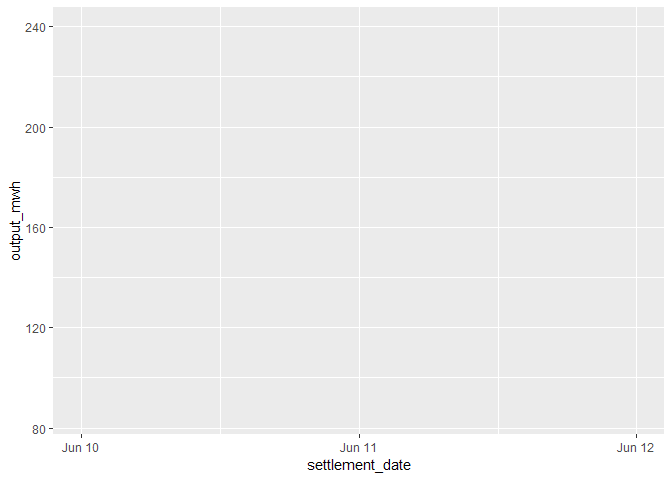
\includegraphics{r_training_tidyverse_files/figure-latex/ggplot2_data_2-1.pdf}

\begin{itemize}
\tightlist
\item
  Here, we've defined our data set and our aesthetics (our mappings),
  but no geometric object
\item
  From this, we could create any type of graph we want
\end{itemize}

\subsection{ggplot2 - layer}\label{ggplot2---layer-2}

\begin{itemize}
\tightlist
\item
  To add a geometric object, we use the appropriate geom\_x function for
  the plot we want\ldots{}
\end{itemize}

\begin{Shaded}
\begin{Highlighting}[]
\KeywordTok{ggplot}\NormalTok{(}\DataTypeTok{data =}\NormalTok{ output_data, }\KeywordTok{aes}\NormalTok{(}\DataTypeTok{x =}\NormalTok{ settlement_date, }\DataTypeTok{y =}\NormalTok{ output_mwh)) }\OperatorTok{+}\StringTok{ }\KeywordTok{geom_point}\NormalTok{()}
\end{Highlighting}
\end{Shaded}

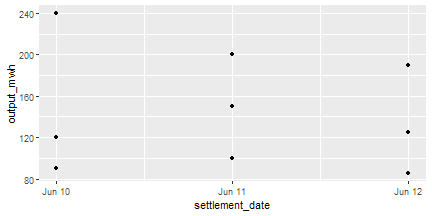
\includegraphics{r_training_tidyverse_files/figure-latex/ggplot2_geom-1.pdf}

\begin{itemize}
\tightlist
\item
  The geom\_point function inherits from our ggplot call, so it knows
  what dataset and X and Y values we want
\item
  And that's a layer completed
\end{itemize}

\subsection{ggplot - structure}\label{ggplot---structure}

\begin{itemize}
\tightlist
\item
  In the previous example, we only had 1 layer
\item
  In some cases however, you may want many layers with different
  aesthetic mappings (particularly if you're grouping)
\item
  By default, each geometric object function inherits the parameters of
  our ggplot call, but you can define additional aesthetics very
  easily\ldots{}
\end{itemize}

\begin{Shaded}
\begin{Highlighting}[]
\KeywordTok{ggplot}\NormalTok{(}\DataTypeTok{data =}\NormalTok{ output_data, }\KeywordTok{aes}\NormalTok{(}\DataTypeTok{x =}\NormalTok{ settlement_date, }\DataTypeTok{y =}\NormalTok{ output_mwh)) }\OperatorTok{+}\StringTok{ }\KeywordTok{geom_point}\NormalTok{() }\OperatorTok{+}\StringTok{ }\KeywordTok{geom_line}\NormalTok{(}\KeywordTok{aes}\NormalTok{(}\DataTypeTok{color =}\NormalTok{ fuel_type))}
\end{Highlighting}
\end{Shaded}

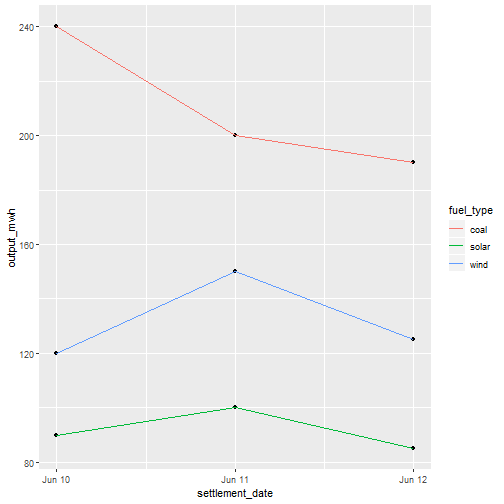
\includegraphics{r_training_tidyverse_files/figure-latex/ggplot2_structure_2-1.pdf}

\subsection{ggplot - structure}\label{ggplot---structure-1}

\begin{itemize}
\tightlist
\item
  Because of how inheritance works in ggplot2, we could produce exactly
  the same graph with\ldots{}
\end{itemize}

\begin{Shaded}
\begin{Highlighting}[]
\KeywordTok{ggplot}\NormalTok{(}\DataTypeTok{data =}\NormalTok{ output_data) }\OperatorTok{+}\StringTok{ }\KeywordTok{geom_point}\NormalTok{(}\KeywordTok{aes}\NormalTok{(}\DataTypeTok{x =}\NormalTok{ settlement_date, }\DataTypeTok{y =}\NormalTok{ output_mwh)) }\OperatorTok{+}\StringTok{ }\KeywordTok{geom_line}\NormalTok{(}\KeywordTok{aes}\NormalTok{(}\DataTypeTok{x =}\NormalTok{ settlement_date, }\DataTypeTok{y =}\NormalTok{ output_mwh, }\DataTypeTok{color =}\NormalTok{ fuel_type))}
\end{Highlighting}
\end{Shaded}

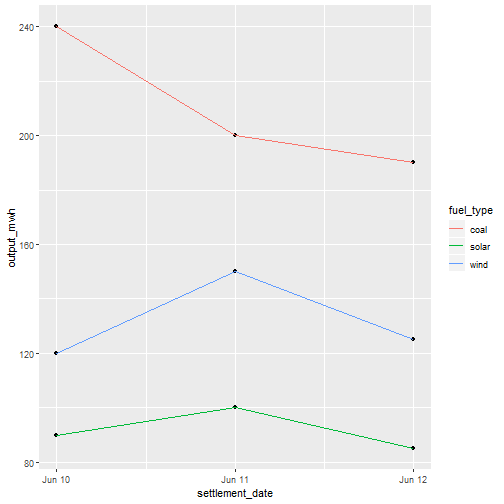
\includegraphics{r_training_tidyverse_files/figure-latex/ggplot2_structure-1.pdf}

\begin{itemize}
\tightlist
\item
  But clearly one is easier to read than the other\ldots{}
\end{itemize}

\subsection{ggplot2 - structure}\label{ggplot2---structure}

\begin{itemize}
\tightlist
\item
  ggplot2 separates out the values and the type of plot you're producing
  (the geometric object)
\item
  This means you can easily change the look of your graph without
  changing the underlying data
\item
  However, some geometric objects can only accept certain aesthetic
  mappings\ldots{}
\end{itemize}

\begin{Shaded}
\begin{Highlighting}[]
\KeywordTok{ggplot}\NormalTok{(}\DataTypeTok{data =}\NormalTok{ output_data) }\OperatorTok{+}\StringTok{ }\KeywordTok{geom_histogram}\NormalTok{(}\KeywordTok{aes}\NormalTok{(}\DataTypeTok{x =}\NormalTok{ output_mwh))}
\end{Highlighting}
\end{Shaded}

\begin{verbatim}
## `stat_bin()` using `bins = 30`. Pick better value with `binwidth`.
\end{verbatim}

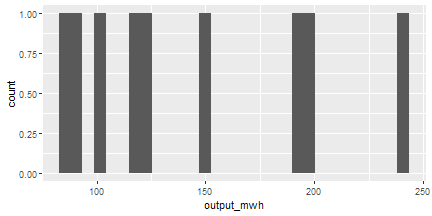
\includegraphics{r_training_tidyverse_files/figure-latex/hist_example-1.pdf}

\begin{itemize}
\tightlist
\item
  There's no Y value for a histogram, so supplying one would give an
  error
\end{itemize}

\subsection{ggplot2 - exercise}\label{ggplot2---exercise}

\begin{itemize}
\tightlist
\item
  Using your tidy data, produce a plot including a grouping variable
\end{itemize}

\subsection{ggplot2 - scales}\label{ggplot2---scales}

\begin{itemize}
\tightlist
\item
  The default scales in ggplot2 are usually pretty good
\item
  However, there will always be aspects that you want to change
\item
  To change a scale, we use the scale\_x\_datatype functions\ldots{}
\end{itemize}

\begin{Shaded}
\begin{Highlighting}[]
\NormalTok{... }\OperatorTok{+}\StringTok{ }\KeywordTok{scale_x_continuous}\NormalTok{()}
\NormalTok{... }\OperatorTok{+}\StringTok{ }\KeywordTok{scale_x_date}\NormalTok{()}
\NormalTok{... }\OperatorTok{+}\StringTok{ }\KeywordTok{scale_x_discrete}\NormalTok{()}
\end{Highlighting}
\end{Shaded}

\subsection{ggplot2 - scales}\label{ggplot2---scales-1}

\begin{itemize}
\tightlist
\item
  Each of these scale\_x\_datatype function accept slightly different
  parameters, but there are some common ones\ldots{}

  \begin{itemize}
  \tightlist
  \item
    name; character string with the scale title
  \item
    breaks; a vector of the scale breaks
  \item
    labels; a vector of character strings the same length as breaks
  \item
    limits; a two value numeric vector
  \item
    expand; a two value numeric vector
  \end{itemize}
\end{itemize}

\subsection{ggplot2 - exercise}\label{ggplot2---exercise-1}

\begin{itemize}
\tightlist
\item
  Change some aspect(s) of both of the scales on your plot
\end{itemize}

\subsection{ggplot2 - themes}\label{ggplot2---themes}

\begin{itemize}
\tightlist
\item
  In ggplot2, we can add themes to our plots
\item
  This changes some of the less important graphical features of the
  graph

  \begin{itemize}
  \tightlist
  \item
    the plotting background color
  \item
    the font
  \item
    the gridlines
  \item
    the text rotation
  \item
    the text size
  \end{itemize}
\item
  Currently, I've got a theme\_elexon(), but it needs some improvement
  so suggestions are welcome
\end{itemize}

\subsection{Conclusion}\label{conclusion}

\begin{itemize}
\tightlist
\item
  The tidyverse is a collection of packages to help with data
  manipulation
\item
  Use tidyr for cleaning, dplyr for manipulation, and ggplot2 for
  plotting
\item
  All packages use a common philosophy, pioneered by Hadley Wickham
\item
  All packages are open source, and very well documented on Github
\end{itemize}


\end{document}
